\subsection{Quarks}

In the mid-20th century, the field of particle physics faced mounting evidence suggesting that protons and neutrons were not elementary particles but had a more complex internal structure.
Enter the quarks.
The concept of quarks was introduced by Murray Gell-Mann and George Zweig independently in 1964.
According to Gell-Mann's model, protons and neutrons are composed of three quarks each.
This was a significant departure from the previously held notion that protons and neutrons were indivisible.

Gell-Mann's model was initially motivated by the observation of patterns among the particles known as baryons and mesons.
Baryons (like protons and neutrons) were seen as composed of triplets of quarks, while mesons were seen as quark-antiquark pairs.

Around the same time, George Zweig proposed a similar idea independently, also introducing the concept of quarks.
Zweig's model was termed the ``Eightfold Way'' and shared many similarities with Gell-Mann's model, though with some differences in the details.

The hypothesis of quarks gained experimental support in the 1970s with deep inelastic scattering experiments conducted at the Stanford Linear Accelerator Center (SLAC).
These experiments probed the internal structure of protons by bombarding them with high-energy electrons.
The results showed evidence of point-like particles within the protons, consistent with the quark model.
The observed scaling behavior of the structure functions in these experiments provided strong evidence for the existence of quarks and their confinement within protons and neutrons.

\begin{figure}[H]
  % https://en.wikipedia.org/wiki/Quark#/media/File:Quark_structure_proton.svg
  \centering
  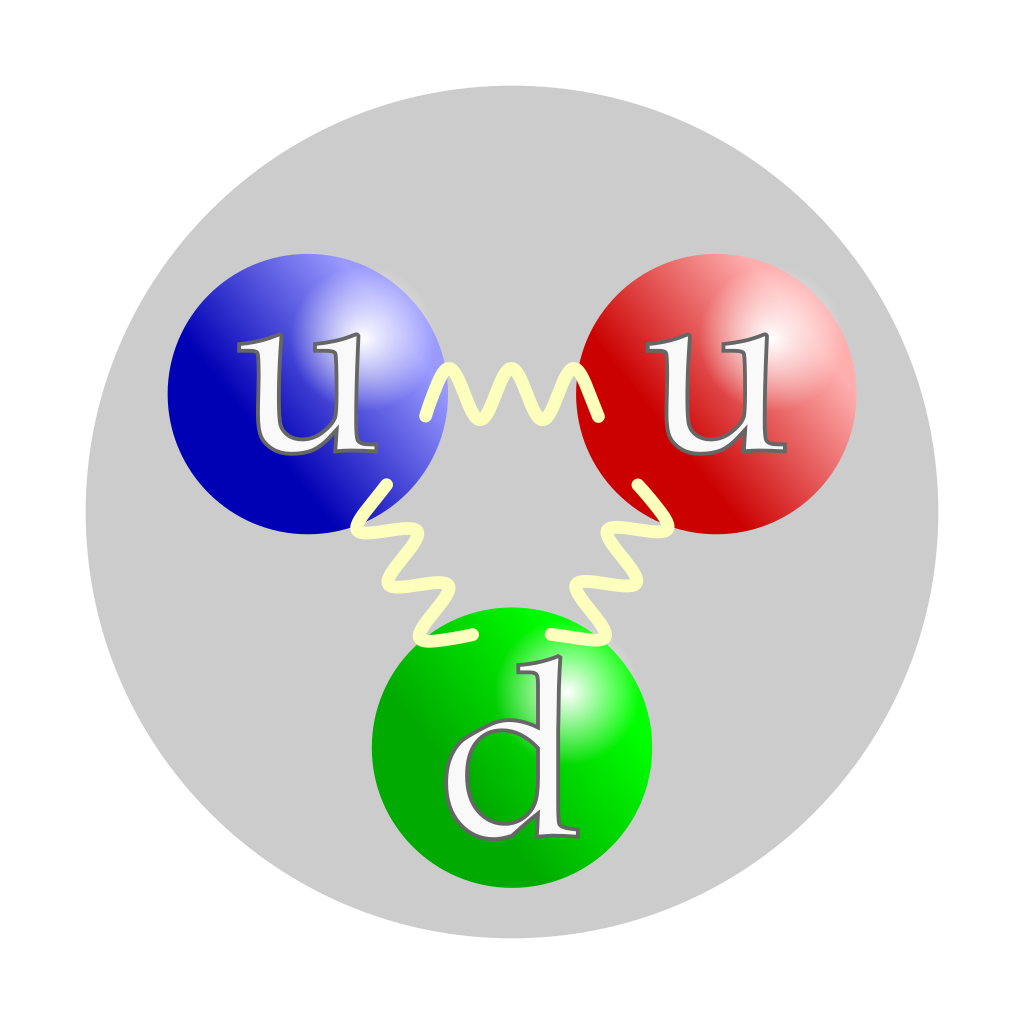
\includegraphics[width=100mm]{figures/protonQuarks.png}
  \caption{Quarks inside a proton.
    Labelled u for up and d for down}
  \label{protonQuarks}
\end{figure}

Further confirmation of the quark model came from the discovery of additional types of quarks and the development of Quantum Chromodynamics (QCD).
QCD provided a comprehensive framework for understanding how quarks are bound together.

Today, quarks are understood to be fundamental constituents of matter, forming the building blocks of protons, neutrons, and other hadrons (Composite subatomic particles that are made up of at least 2 quarks).

We have so far discovered 6 flavors of quarks -- up (\(u\)), down (\(d\)), charm (\(c\)), strange (\(s\)), top (\(t\)), and bottom (\(b\)).
Each flavor has different mass.
These masses and their interactions with other particles are crucial for the stability and properties of atomic nuclei.

\begin{table}[h!]
  % Could you please check if the numbers in the table are correct, I'm not 100 percent sure
  \centering
  \begin{tabular}{lrr}
    \toprule
    Quark Flavor & Approximate Mass (MeV/c\(^2\)) & Charge (e) \\
    \midrule
    Up (u)      & 2.2 - 3.0        & +\(\frac{2}{3}\) \\
    Down (d)    & 4.7 - 5.0        & -\(\frac{1}{3}\) \\
    Strange (s) & 95 - 105         & -\(\frac{1}{3}\) \\
    Charm (c)   & 1270 - 1720      & +\(\frac{2}{3}\) \\
    Bottom (b)  & 4180 - 4380      & -\(\frac{1}{3}\) \\
    Top (t)     & 172000 - 173000  & +\(\frac{2}{3}\) \\
    \bottomrule
  \end{tabular}
  \caption{Quark Flavors and Their Approximate Masses}
  \label{quarkMass}
\end{table}

Quarks carry fractional electric charges.
For instance, up quarks have a charge of \(+\frac{2}{3}\) e, while down quarks have a charge of \(-\frac{1}{3}\) e, where e is the elementary charge.
This fractional charge is essential for the charge balance in particles such as protons and neutrons.

Quarks are never found in isolation due to a phenomenon known as confinement.
They are always confined within larger particles called hadrons.

Quarks have a property called color charge, analogous to electric charge but related to the strong force.
There are three types of color charges: red, green, and blue.
The strong interaction, which is described by QCD, ensures that particles made of quarks are color-neutral.

For each quark flavor, there exists a corresponding antiquark with the opposite charge.
Antiquarks can combine with quarks to form mesons, another category of hadrons.

